\documentclass{resume} % The custom resume.cls style

\usepackage[left=0.75in,top=0.6in,right=0.75in,bottom=0.6in]{geometry} % Document margins
\usepackage{graphicx}
\usepackage[utf8]{inputenc}
\usepackage[T1]{fontenc}
\usepackage[stretch=10]{microtype}
\usepackage{hyperref}
\usepackage{tgpagella}
\usepackage{enumitem}
\usepackage{indentfirst}

\newcommand{\tab}[1]{\hspace{.2667\textwidth}\rlap{#1}}
\newcommand{\itab}[1]{\hspace{0em}\rlap{#1}}

\name{Kartik Vishnu Hegde}

% Address and Contact Section

\begin{document}

\begin{rSection}{}

 S/o Vishnu V Hegde 
 \\Malige Mane, Po: Muroor, Tq : Kumta  
 \\Dist : Uttara Kannada 
 \\Karnataka, 581362\\
 \\Contact : 9482543175
 \\email ID: kartikhegde0611@gmail.com\hfill 
 \raisebox{-.1\totalheight}[0pt][.3\totalheight]{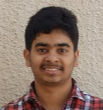
\includegraphics[width=2.5cm,height=2.7cm]{kartik.png}}

\end{rSection}


\vspace{1cm}

% Carrier Objective Section

\begin{rSection}{Carrier Objective}

 To work for an organization which provides me the opportunity to improve my skills and knowledge to grow along with the organization objective. To do significant contribution to the success of the organization.
 
\end{rSection}


\vspace{1cm}


% Education Section 

\begin{rSection}{Education}

\begin{tabular}{ |p{3cm}|p{3cm}|p{3.5cm}|p{2cm}|p{2.5cm}| }

 \hline
 &&&&\\ \textbf{ Course} & \textbf{Discipline} & \textbf{College/School}& \textbf{Passing Year} &  \textbf{Passing}\\
&&&&\textbf{Percentage}\\

 \hline
&&&&\\B.Tech &  Electronics and  &        PES UNIVERSITY &       2020 &         \textbf{8.40} CGPA\\
&Communication&Bangalore&&Sem 1 to 5\\
&Engineering&&&\\

 \hline
&&&&\\Pre University &\textit{Class-12th :} &Alvas PU College& 2016 & 95.5\\
&Karnataka & Moodabidri &&\\
&State Board& &&\\

\hline
&&&&\\School&\textit{Class-10th :}& Pragati Vidyalaya &2014& 94.24\\
&Karnataka& Muroor &&\\
&State Board&Kumta&&\\

\hline
\end{tabular}


\end{rSection}

\vspace{1cm}

\newpage

% Projects Section


\begin{rSection}{Projects}

\begin{enumerate}


\item Built a \textbf{Fruit Plucking robot} for JED-I(Joy of Engineering Design and Innovation) lab using Arduino Uno and image processing using
opencv.

\item \textbf{Sun tracking solar panel} using AT89C51 microcontroller and LDR sensors.

\item \textbf{Cell Phone Detector} using LM358 Dual OpAmp.

\item \textbf{Air Bubble Detector} \textit{for dialysis machine} using Arduino Uno and BH1750 sensor and Adafruit TSL2591 sensor under the guidance of \textit{Dr.Manikandan.J} (CORI, PES University) . 

\item \textbf{Keyboard Playing Robot} as a mini project for the course \textbf{Introduction to Robotics} . (\textit{In progress})

\item Implementation of \textbf{Point of Sale Transaction} using \textit{MFRC522, RFID module}.

\end{enumerate}
\end{rSection}

\vspace{1cm}


\end{document}



